%%This is a very basic article template.
%%There is just one section and two subsections.
\documentclass{article}
\usepackage{graphicx}
\usepackage{cite}
\usepackage{booktabs}
\graphicspath{ {images/} }


\begin{document}

\bibliographystyle{plain}


\section{Title}

\subsection{Introduction}
%introduce whole study and paper here (together)

\subsection{Background}
%literature background (Natalie)

\subsection{Materials and Methods}


The original dataset utilised in this study consists in 1,562 responses from a
quantitative survey conducted on behalf of the ACNC by ChantLink in 2013. It
does not include a pilot phase of 62 responses. The survey collected information
about levels of trust in charities and factors that may affect these levels. The
respondents were asked to rate their level of trust and their agreement with a
series of statements about charities on a scale from 1 to 10. They also were
asked about their involvement, knowledge of charities sector and demographics.
Specifically, the survey was divided into 5 sections: Awareness and Involvement
in Charities, Trust, Regulation, Public Register of Charities and Demographics.

Aiming to cluster the survey respondents according their trust and confidence in
charities, a new dataset was obtained from the original dataset. It consists of
the Trust section responses which were rated on the scale from 1 to 10. In
addition, the questions not answered by all the respondents and those with
user-typed responses were removed. This procedure was adopted in order to select
informative and comparable questions as the survey contains different types of
questions. Overall, 1,562 responses of 43 different questions was considered in
the clustering step.

Since the dataset can be represented as a graph, the methodology utilised for
clustering is based on a novel graph-based clustering algorithm propose by
~\cite{Inostroza2008}. The MSTkNN combines a Minimum Spanning Tree (MST) and a
k-Nearest Neighbor (kNN) proximity graphs. This combination allows us to perform
a graph partitioning operation, which produce a clustering of the dataset
represented by its graph. The graph partitioning separates the data in groups
with similar characteristics utilizing a given proximity measurement. In this
case, the Spearman correlation was used to measure the distance between
different features of the dataset's graph.

Given a undirected and connected graph, a MST is a subgraph which is a tree and
contain all the objects connected by the minimum possible distance between each
other, based on a determined measurement of the distance. Whereas, the kNN graph
is a graph where their objects are connected if they are commutual k nearest
neighbors of each other according to a defined value of k. In this work, the
value of k was defined as 3 for computing the kNN graph. The merge of these
methods permit delete the connection between two objects in the MST if they are
not reciprocally one of the k nearest of each other. Consequently, the MST is
partitioned into smaller subgraphs which are the resultant clusters.

%Normalization by row?

After clustering the dataset, the new score introduced by~\cite{Marsden2013}
was computed to highlight the individual characteristics of each cluster. The
CM1 scores gives a overview about differences in averages for each feature from
a specific cluster in the investigated dataset. The rank of the CM1 scores of a
cluster can be split into top or bottom features. The top features refers to
features whose average are greater in a specific cluster than in all the others,
while bottom refers to features whose average are less in a specific cluster
than in all the others. The CM1 scores are then computed using the following
formula~(\ref{eq:01}).

\begin{equation}
CM1(w,X,Y) = \frac{\frac{1}{\left|X\right|}  \sum_{x \in X} x_{w} - \frac{1}{\left|Y\right|}  \sum_{y \in Y} y_{w}} {1 + max_{y \in Y } \left\{ y_{w} \right\}- min_{y \in Y} \left\{y_{w}\right\} } \label{eq:01}
\end{equation}

%this study was based on the study done in UK and NZ


\subsection{Results}

The MSTkNN clustering algorithm was able to find 7 different clusters of
different sizes according Figure \ref{fig:Clusters}. These included Cluster0
(13\%), Cluster1 (10\%), Cluster2 (12\%), Cluster3 (20\%), Cluster4 (3\%),
Cluster5(36\%) and Cluster6 (6\%).


\begin{figure}[h]
	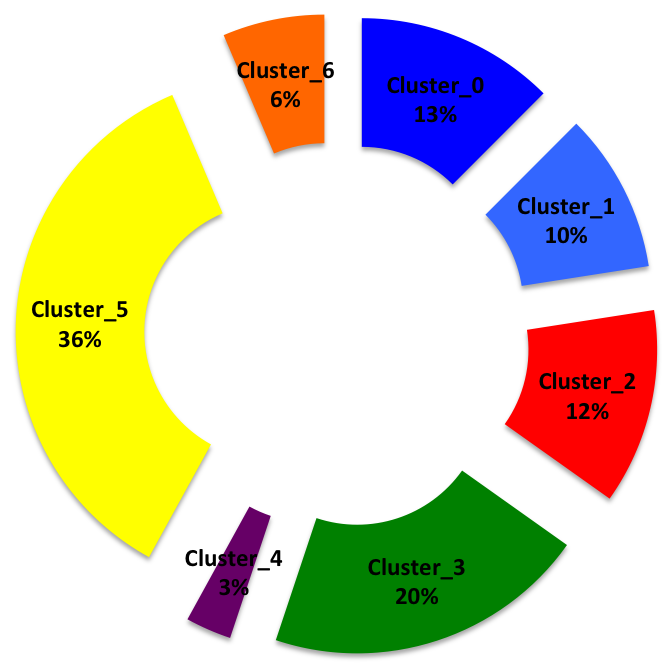
\includegraphics[scale=0.5]{Clusters.png}
	\caption{\textbf{Percentage of respondents for each cluster discovered by the
	MSTkNN clustering algorithm} The MSTkNN.}
	\label{fig:Clusters}
\end{figure}

The CM1 score was calculated for all the 43 features of the new dataset
for each of the discovered clusters. The selected top and bottom features for
each cluster is presented in the Tables~\ref{tab:bottom} and ~\ref{tab:top}.

\begin{table}[htbp]
  \centering
  \caption{Bottom features for each cluster (presented in descending order of
  score)}
    \begin{tabular}{rrrrrrr}
    \toprule
    Cluster\_0 & Cluster\_1 & Cluster\_2 & Cluster\_3 & Cluster\_4 & Cluster\_5 & Cluster6 \\
    \midrule
    Q7B\_7 & Q9\_13 & Q9\_10 & Q11\_6\_1 & Q9\_15 & Q9\_07 & Q11\_1\_1 \\
    Q7B\_11 & Q9\_14 & Q9\_02 & Q11\_5\_1 & Q9\_04 & Q9\_05 & Q11\_5\_1 \\
    Q7B\_9 & Q9\_19 & Q7B\_7 & Q11\_1\_1 & Q9\_16 & Q9\_06 & Q11\_4\_1 \\
    Q7B\_6 & Q9\_10 & Q7B\_6 & Q11\_3\_1 & Q9\_21 & Q9\_20 & Q11\_6\_1 \\
    Q7B\_5 & Q9\_03 & Q9\_03 & Q11\_2\_1 & Q9\_24 & Q9\_21 & Q11\_2\_1 \\
    Q7B\_10 & Q9\_11 & Q9\_23 & Q9\_15 & Q7B\_1 & Q11\_5\_1 & Q11\_3\_1 \\
    Q7B\_3 & Q9\_09 & Q7B\_11 & Q9\_04 & Q9\_25 & Q11\_3\_1 & Q9\_15 \\
    Q9\_09 & Q9\_01 & Q9\_25 &       & Q9\_23 &       & Q9\_04 \\
    Q9\_02 & Q7A   & Q9\_19 &       & Q7B\_2 &       &  \\
    Q9\_10 & Q9\_12 & Q9\_22 &       & Q9\_20 &       &  \\
    Q7B\_4 & Q9\_18 & Q7A   &       & Q9\_22 &       &  \\
    Q7B\_8 & Q9\_23 & Q9\_24 &       &       &       &  \\
          &       & Q9\_08 &       &       &       &  \\
    \bottomrule
    \end{tabular}
  \label{tab:bottom}
\end{table}


\begin{table}[htbp]
  \centering
  \caption{Top features for each cluster (presented in descending order of
  score)}
    \begin{tabular}{rrrrrrr}
    \toprule
    Cluster\_0 & Cluster\_1 & Cluster\_2 & Cluster\_3 & Cluster\_4 & Cluster\_5 & Cluster6 \\
    \midrule
    Q11\_1\_1 & Q11\_4\_1 & Q11\_4\_1 & Q9\_19 & Q7B\_4 & Q9\_12 & Q7B\_1 \\
    Q9\_07 & Q11\_2\_1 & Q11\_1\_1 & Q9\_03 & Q11\_2\_1 & Q9\_08 & Q7B\_9 \\
    Q11\_6\_1 & Q11\_1\_1 & Q9\_20 & Q7A   & Q7B\_3 & Q9\_01 & Q7B\_8 \\
    Q9\_25 & Q11\_6\_1 & Q9\_21 & Q7B\_11 & Q9\_02 & Q9\_16 & Q9\_10 \\
    Q9\_22 & Q11\_3\_1 & Q11\_6\_1 & Q7B\_7 & Q9\_10 & Q9\_11 & Q7B\_10 \\
    Q9\_05 & Q11\_5\_1 & Q11\_3\_1 & Q9\_09 & Q11\_1\_1 & Q9\_03 & Q7B\_2 \\
    Q11\_3\_1 & Q9\_20 & Q11\_5\_1 & Q9\_10 & Q11\_4\_1 & Q9\_19 & Q7B\_5 \\
    Q9\_06 & Q9\_21 & Q9\_06 & Q9\_02 & Q11\_5\_1 & Q9\_13 & Q7B\_7 \\
    Q11\_5\_1 & Q9\_05 & Q9\_05 &       &       & Q9\_14 & Q9\_02 \\
    Q9\_24 & Q9\_06 & Q9\_07 &       &       &       & Q7B\_3 \\
    Q9\_20 & Q9\_07 &       &       &       &       & Q7B\_11 \\
    Q9\_23 &       &       &       &       &       & Q7B\_6 \\
    Q9\_21 &       &       &       &       &       & Q7B\_4 \\
    \bottomrule
    \end{tabular}
  \label{tab:top}
\end{table}



% Cluster 0

The Figure~\ref{fig:CM1Cluster0} demonstrate the CM1 score for the 43 features
for Cluster0, with the 12 bottom and 13 top features shown in red and green
respectively. The question Q7B, which aims to rate the trust and confidence
levels between different institutions and organizations, is shown to dominate as
a bottom features, representing 9 of them. Among the top features, the
questions Q11 which rate the importance for charities providing some types of
information and Q9 that rate the respondents agreement with factors that may
drive trust in charities are shown as a positive features. The difference
between the cumulative CM1 scores for the top and bottom features for Cluster0
is shown in the Figure~\ref{fig:DifferencesCluster0}. It shows a proximity
between Cluster0, Cluster1 and Cluster2 which score higher positive results
against these features.


\begin{figure}[h]
	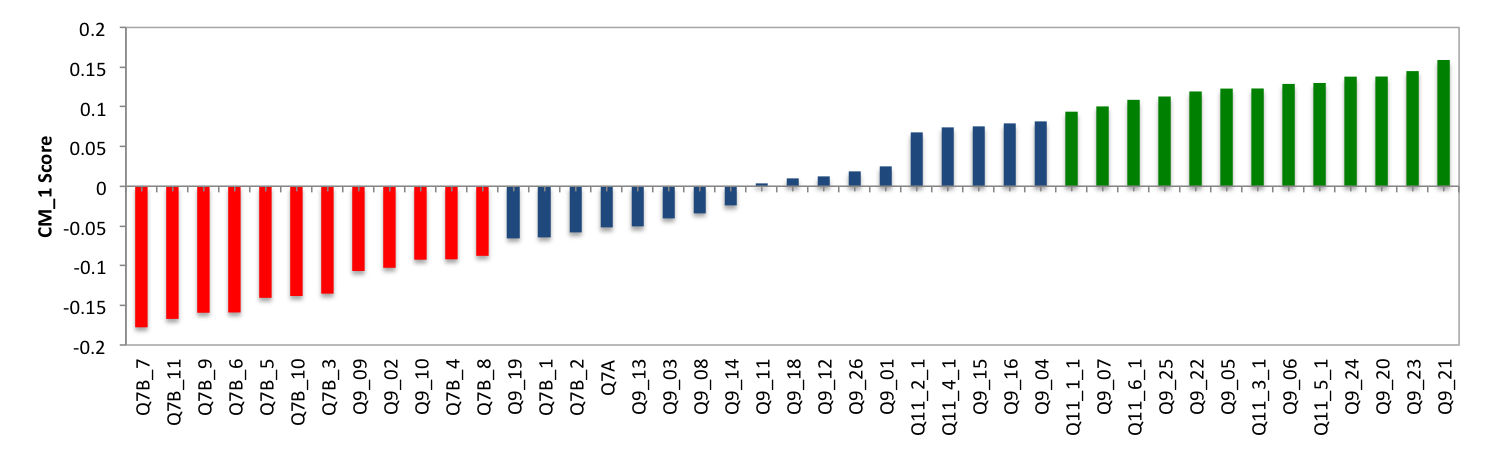
\includegraphics[ width=\textwidth ]{CM1_Cluster0.png}
	\caption{CM1 Scores for the 43 features for Cluster0, based on the new dataset.
	The selected top and bottom features are shown in red and green respectively
	and are presented in Tables~\ref{tab:bottom} and~\ref{tab:top}. The majority of
	bottom features are from question Q7B which suggests lower rates of trust and
	confidence in specific institutions and organizations.}
	\label{fig:CM1Cluster0}
\end{figure}
\begin{figure}[h]
	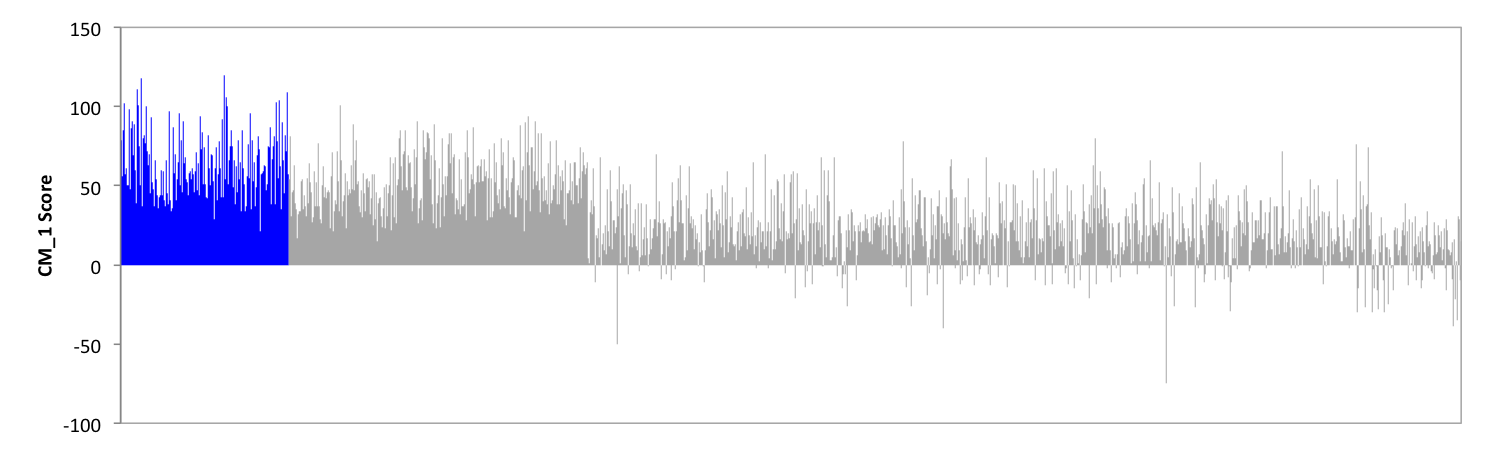
\includegraphics[ width=\textwidth]{Difference_Cluster0.png}
	\caption{Difference between the cumulative CM1 scores for the 12 bottom and 13
	top features for Cluster0, as presented in Tables~\ref{tab:bottom}
	and~\ref{tab:top}. The respondents of Cluster0 are shown in blue. It is
	observed that they score higher positive, and they score relatively
	close to Cluster1 and Cluster2.}
	\label{fig:DifferencesCluster0}
\end{figure}

% Cluster 1

The 12 bottom and 11 top CM1 scores for the 43 features for Cluster1 are shown
in red and green respectively in Figure~\ref{fig:CM1Cluster1}. The bottom
features consists mainly by features from question Q9 with Q7A as the only
exception. The question Q7A rates the trust and confidence in Australian
charities overall and only appears as bottom feature for this cluster and
Cluster2. The question Q11 which is related with the information provided by
charities appears as a significant question among the top features. The
difference between cumulative CM1 scores for these top and bottom features for
Cluster1 is shown in the Figure~\ref{fig:DifferencesCluster1}. It confirms a
proximity between Cluster1 and Cluster2, and it also shows that these
two clusters score positive results against these features.


\begin{figure}[h]
	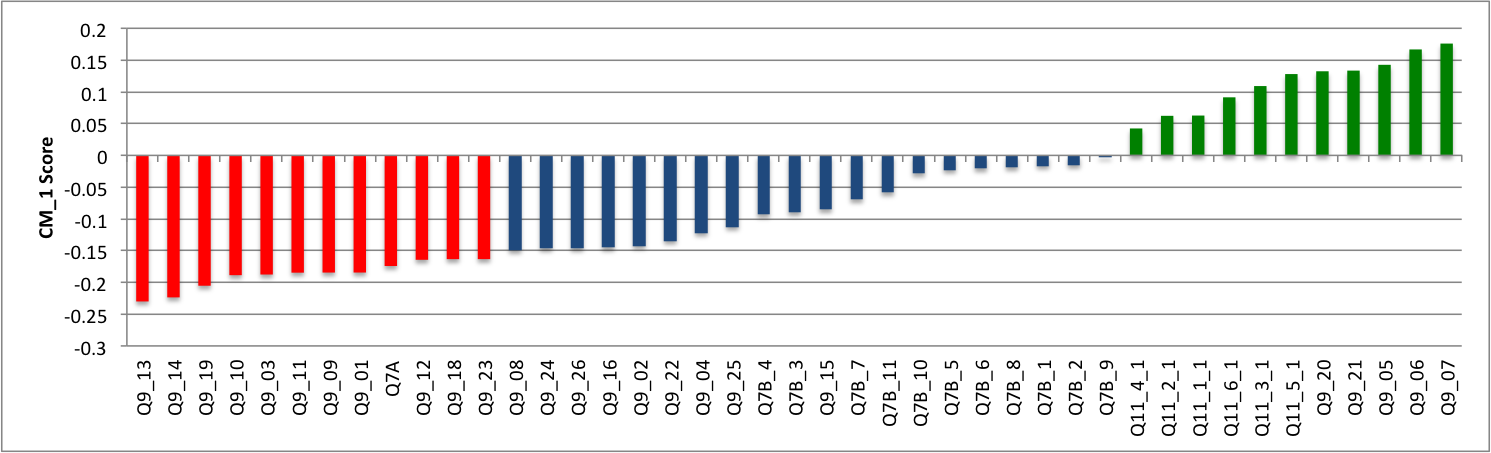
\includegraphics[ width=\textwidth ]{CM1_Cluster1.png}
	\caption{CM1 Scores for the 43 features for Cluster1, based on the new dataset.
	The selected top and bottom features are shown in red and green respectively
	and are presented in Tables~\ref{tab:bottom} and~\ref{tab:top}. The majority of
	top features are from question Q11 which suggests that the respondents from
	this group priority care about the information that Australian charities
	provide.}
	\label{fig:CM1Cluster1}
\end{figure}
\begin{figure}[h]
	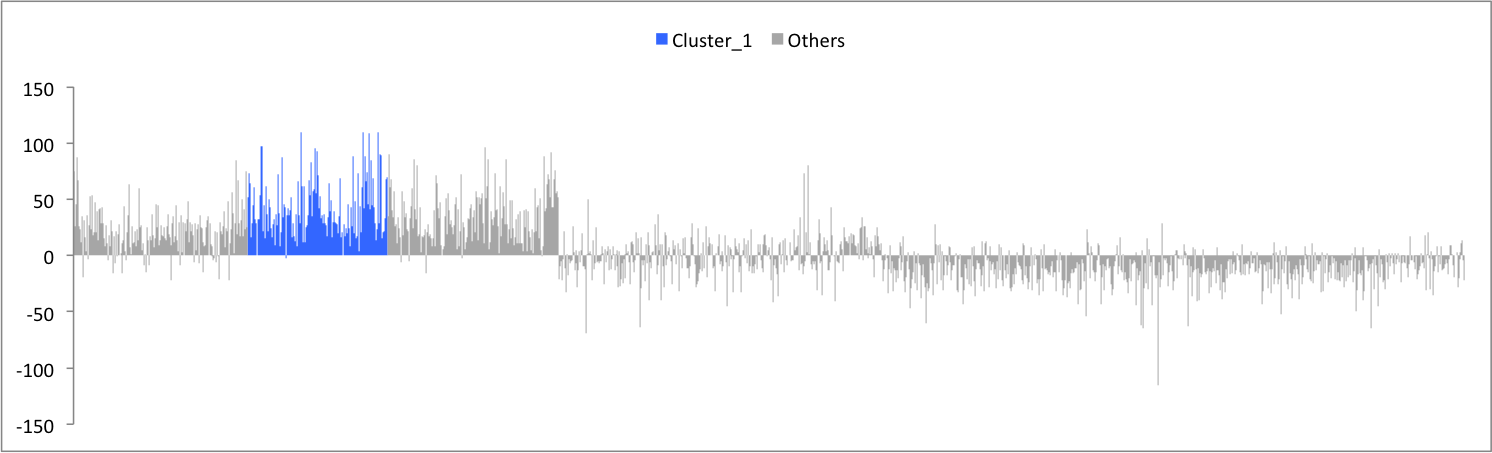
\includegraphics[ width=\textwidth]{Difference_Cluster1.png}
	\caption{Difference between the cumulative CM1 scores for the 12 bottom and 13
	top features for Cluster1, as presented in Tables~\ref{tab:bottom}
	and~\ref{tab:top}. The respondents of Cluster1 are shown in light blue. It is
	observed that they score higher results against these features and are
	relatively close from the respondents of Cluster2.}
	\label{fig:DifferencesCluster1}
\end{figure}

% Cluster 2

Figure~\ref{fig:CM1Cluster2} shows the 13 bottom and 11 top CM1 scores for
Cluster2 in red and green respectively. The questions Q9, Q7B and Q7A compose
the bottom features for this cluster and the questions Q11 and Q9 the top
features. Figure~\ref{fig:DifferencesCluster2} shows the difference between
the cumulative CM1 scores for these features for Cluster2. It is observed that
the majority of the respondents of this cluster, and also Cluster1, score
more positive results against these features.

\begin{figure}[h]
	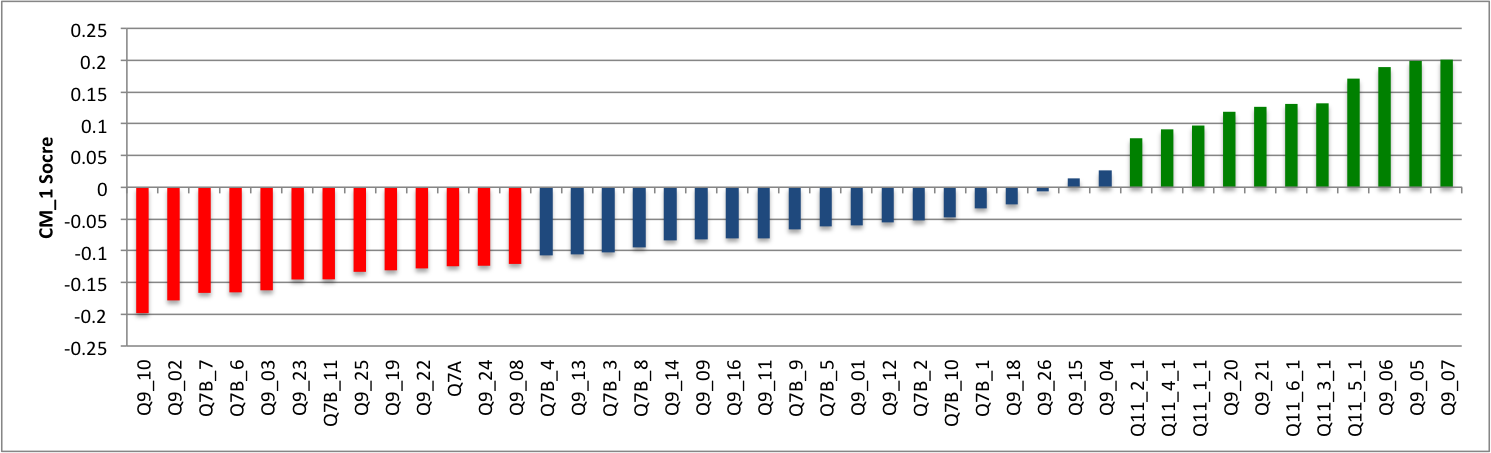
\includegraphics[ width=\textwidth ]{CM1_Cluster2.png}
	\caption{CM1 Scores for the 43 features for Cluster2, based on the new dataset.
	The selected top and bottom features are shown in red and green respectively
	and are presented in Tables~\ref{tab:bottom} and~\ref{tab:top}. The bottom
	features are composed by features from questions Q9, Q7B and Q7A that
	suggests a low rate of trust and confidence in Australian charities overall
	and specific institutions and organizations. On the other hand, The top
	features are composed by questions Q11 and Q9 features that suggest a
	greater concern about the information disponibilizide by charities.}
	\label{fig:CM1Cluster2}
\end{figure}
\begin{figure}[h]
	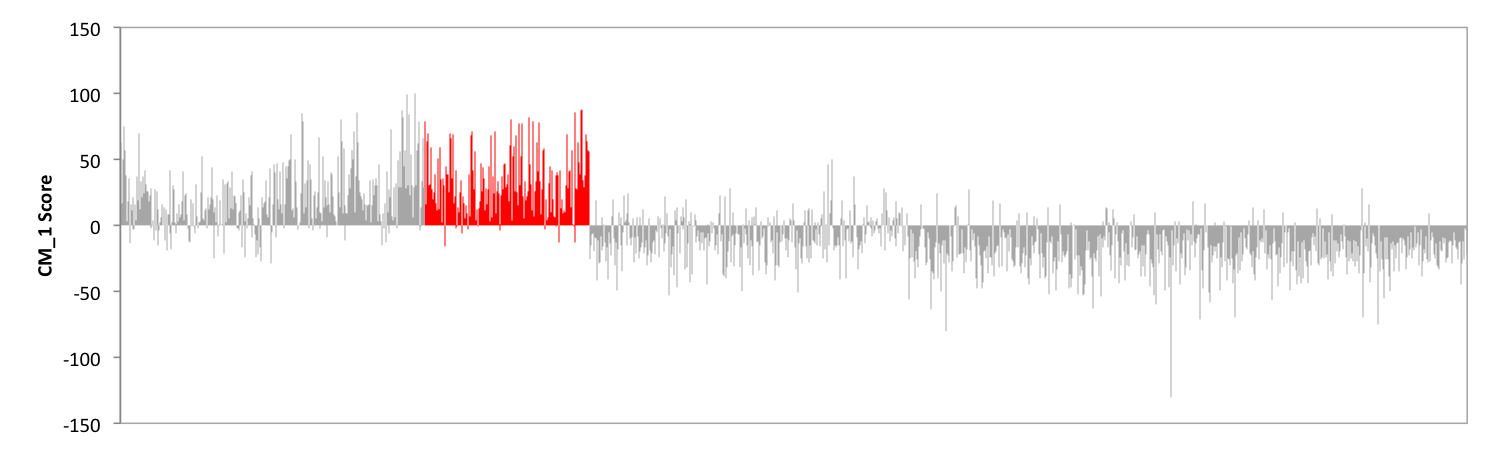
\includegraphics[ width=\textwidth]{Difference_Cluster2.png}
	\caption{Difference between the cumulative CM1 scores for the 13 bottom and 11
	top features for Cluster2, as presented in Tables~\ref{tab:bottom}
	and~\ref{tab:top}. The respondents of Cluster2 are shown in red. It is
	observed that they score higher results against these features and are
	relatively close from the respondents of Cluster1.}
	\label{fig:DifferencesCluster2}
\end{figure}

% Cluster 3

Figure~\ref{fig:CM1Cluster3} shows the 7 bottom and 8 top features for Cluster3
in red and green respectively. Contrary Cluster1 and Cluster 2, the Q11 features
appears as the most negative ranked features for this cluster. This question
aims to rate the importance of Australian charities providing some kinds of
information. The top features consist of features from the Q9, Q7A and Q7B
questions. The question Q7A is observed as a top feature, and this question is
only present in this cluster as a top feature. The difference between the
cumulative CM1 scores for the top and bottom features are shown in
Figure~\ref{fig:DifferencesCluster3}. The respondents of Cluster3 score less
negative results against these features compared mainly to Cluster0, Cluster1
and Cluster2.

\begin{figure}[h]
	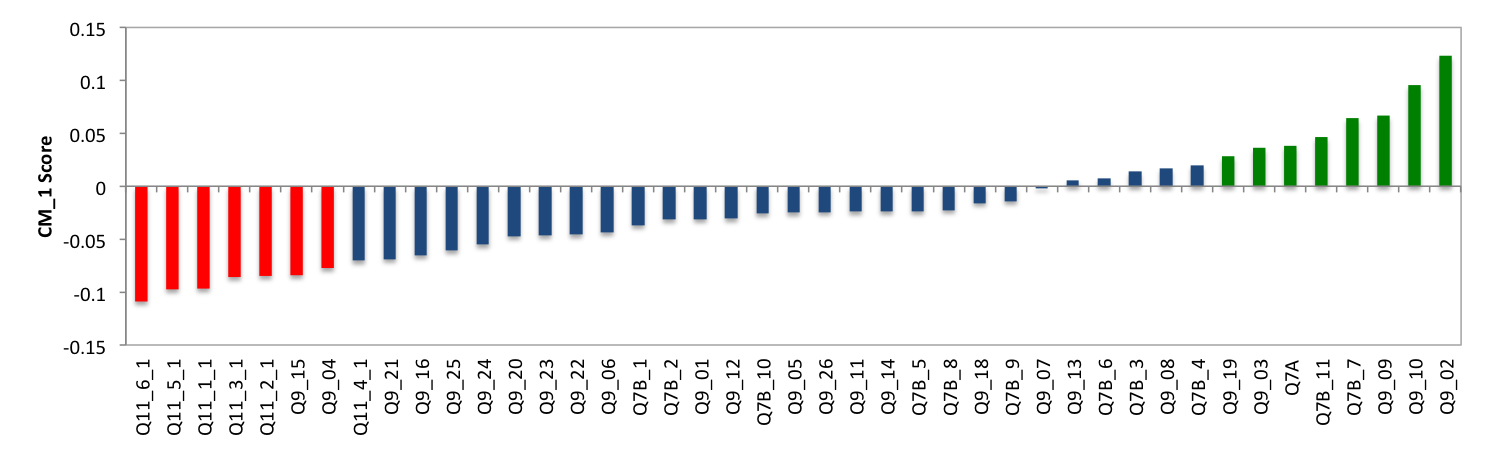
\includegraphics[ width=\textwidth ]{CM1_Cluster3.png}
	\caption{CM1 Scores for the 43 features for Cluster3, based on the new dataset.
	The selected top and bottom features are shown in red and green respectively
	and are presented in Tables~\ref{tab:bottom} and~\ref{tab:top}. The
	most negative ranked features are from question Q11 that suggests a low
	interest in the information that charities may provide. The questions Q7A and
	Q7B among the most positive ranked questions indicate a high rate of trust and
	confidence in charities.}
	\label{fig:CM1Cluster3}
\end{figure}
\begin{figure}[h]
	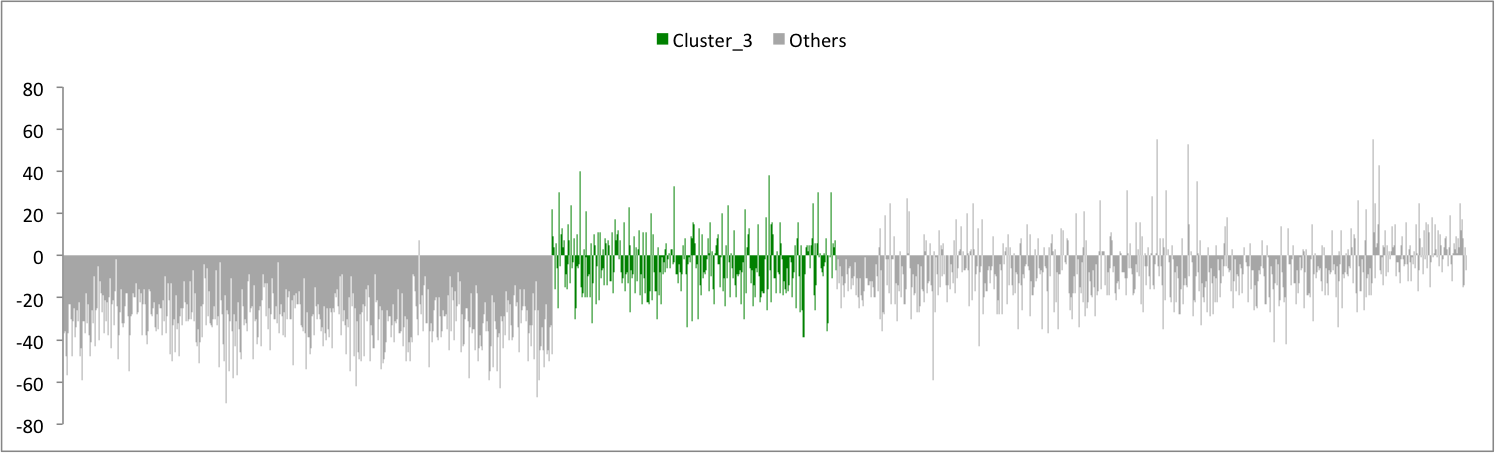
\includegraphics[ width=\textwidth]{Difference_Cluster3.png}
	\caption{Difference between the cumulative CM1 scores for the 7 bottom and 8
	top features for Cluster3, as presented in Tables~\ref{tab:bottom}
	and~\ref{tab:top}. The respondents of Cluster3 are shown in green. It is
	observed that they score less negative results against these features
	compared mainly to the previous clusters.}
	\label{fig:DifferencesCluster3}
\end{figure}

% Cluster 4

The Figure~\ref{fig:CM1Cluster4} demonstrate the CM1 score for the 43 features
for Cluster4, with the 11 bottom and 8 top features shown in red and green
respectively. The question Q9 dominate as a bottom feature and the questions
Q7, Q11 and Q9 among the top features. The difference between the cumulative
CM1 scores for the top and bottom features for Cluster0 is shown in the
Figure~\ref{fig:DifferencesCluster4}. It is observed that the respondents of
Cluster4 score less negative results against these features.

\begin{figure}[h]
	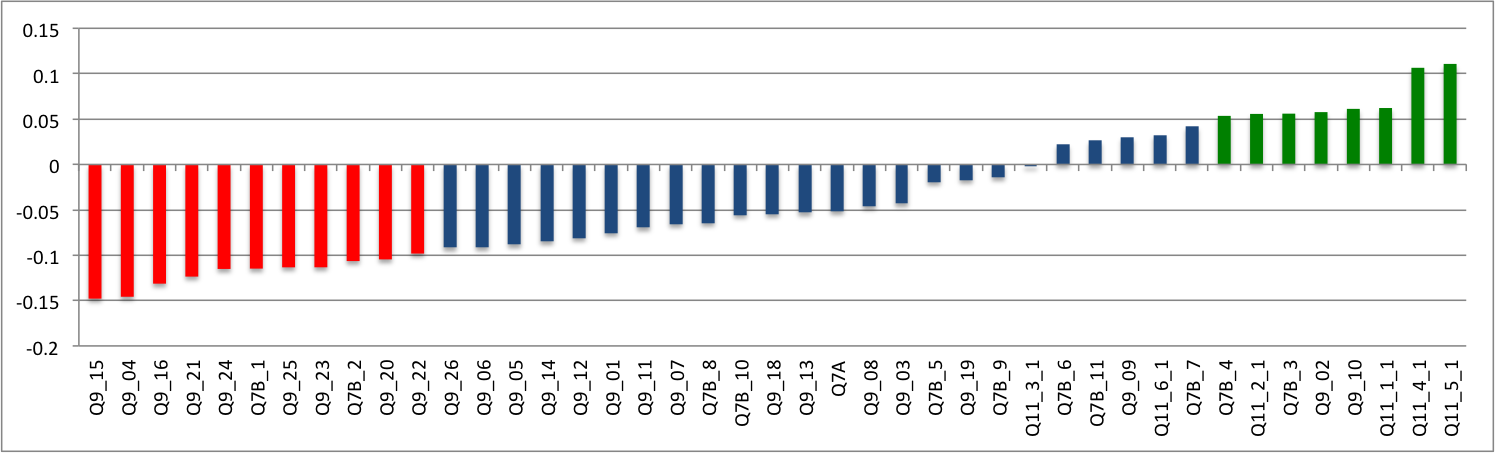
\includegraphics[ width=\textwidth ]{CM1_Cluster4.png}
	\caption{CM1 Scores for the 43 features for Cluster4, based on the new dataset.
	The selected top and bottom features are shown in red and green respectively
	and are presented in Tables~\ref{tab:bottom} and~\ref{tab:top}. The bottom
	features for Cluster4 consist mostly of Q9 features, and the top features
	consist of the questions Q7B, Q11 and Q9 features.}
	\label{fig:CM1Cluster4}
\end{figure}
\begin{figure}[h]
	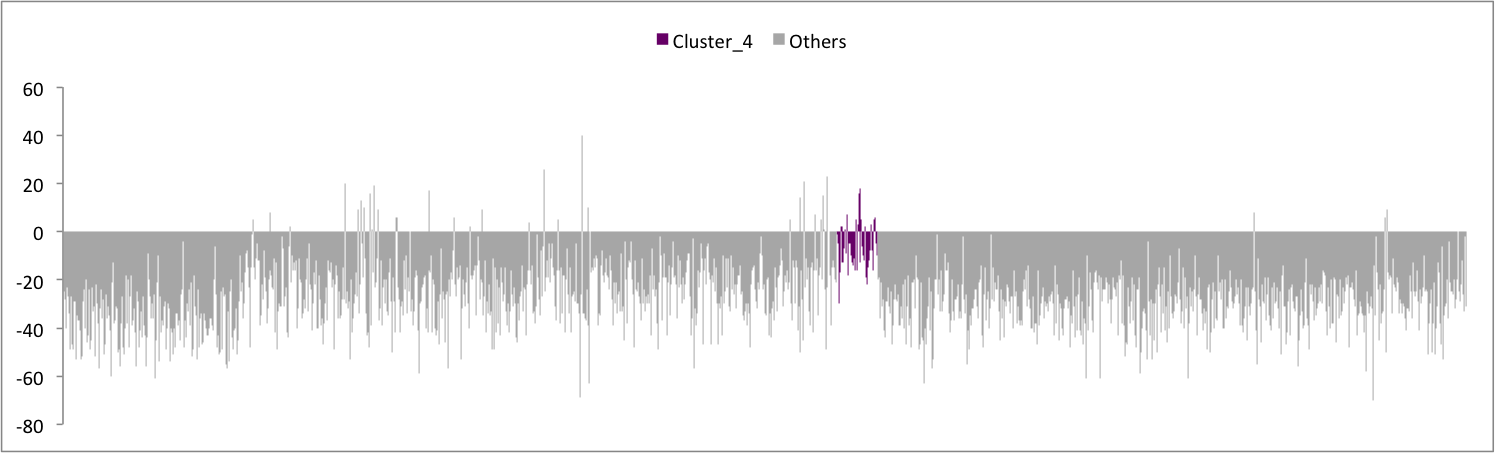
\includegraphics[ width=\textwidth]{Difference_Cluster4.png}
	\caption{Difference between the cumulative CM1 scores for the 11 bottom and 8
	top features for Cluster4, as presented in Tables~\ref{tab:bottom}
	and~\ref{tab:top}. The respondents of Cluster4 are shown in dark purple. It is
	observed that they score less negative results against these features}
	\label{fig:DifferencesCluster4}
\end{figure}

% Cluster 5

Figure~\ref{fig:CM1Cluster5} shows the 7 bottom and 9 top features for Cluster5
in red and green respectively. The Q9 question is the most ranked question in
both, bottom and top features. This fact might highlight important factors that
affect trust and confidence since the Cluster5 is the biggest cluster,
representing 36\% of all respondents. The difference between the
cumulative CM1 scores for the top and bottom features are shown in
Figure~\ref{fig:DifferencesCluster3}. It is observed that the respondents of
Cluster5 score strong positive results against these feature.

\begin{figure}[h]
	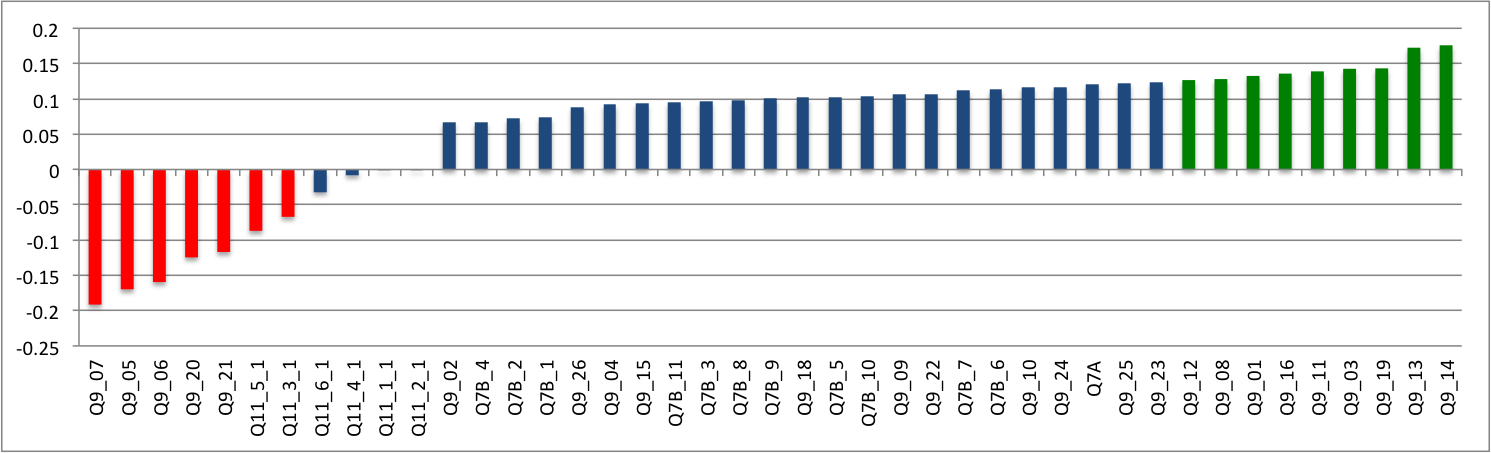
\includegraphics[ width=\textwidth ]{CM1_Cluster5.png}
	\caption{CM1 Scores for the 43 features for Cluster5, based on the new dataset.
	The selected top and bottom features are shown in red and green respectively
	and are presented in Tables~\ref{tab:bottom} and~\ref{tab:top}. Since
	Cluster5 is the biggest cluster and the question Q9 represents the most ranked
	bottom and top features, may it help to identify important factors that
	influence the trust and confidence rate.}
	\label{fig:CM1Cluster5}
\end{figure}
\begin{figure}[h]
	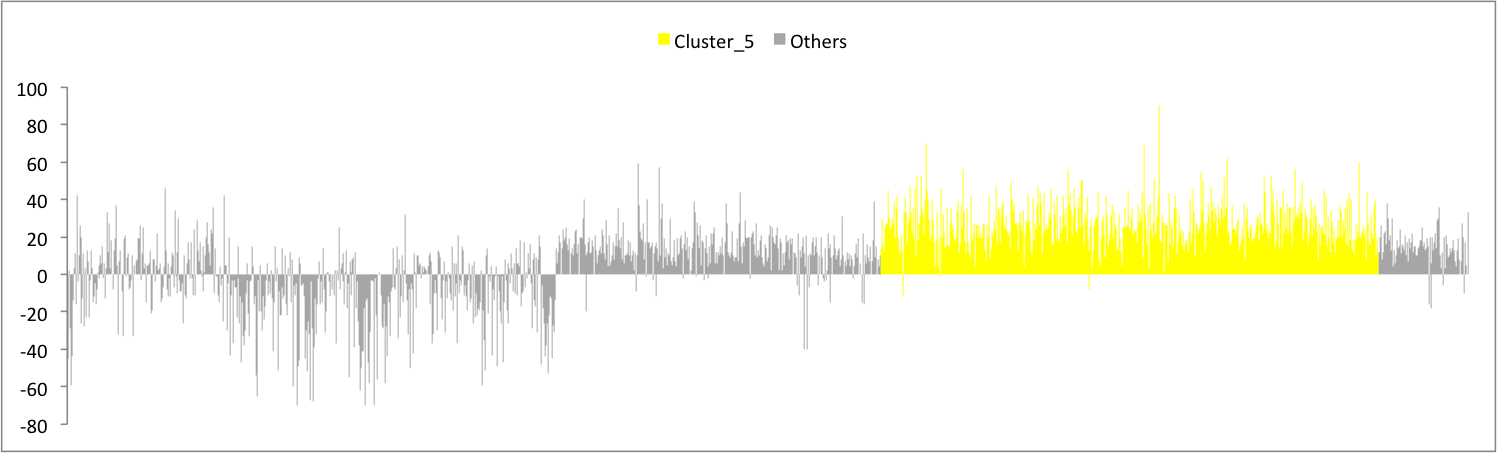
\includegraphics[ width=\textwidth]{Difference_Cluster5.png}
	\caption{Difference between the cumulative CM1 scores for the 7 bottom and 9
	top features for Cluster5, as presented in Tables~\ref{tab:bottom}
	and~\ref{tab:top}. The respondents of Cluster5 are shown in dark yellow. It is
	observed that they score strong positive results against these features}
	\label{fig:DifferencesCluster5}
\end{figure}

% Cluster 6

\begin{figure}[h]
	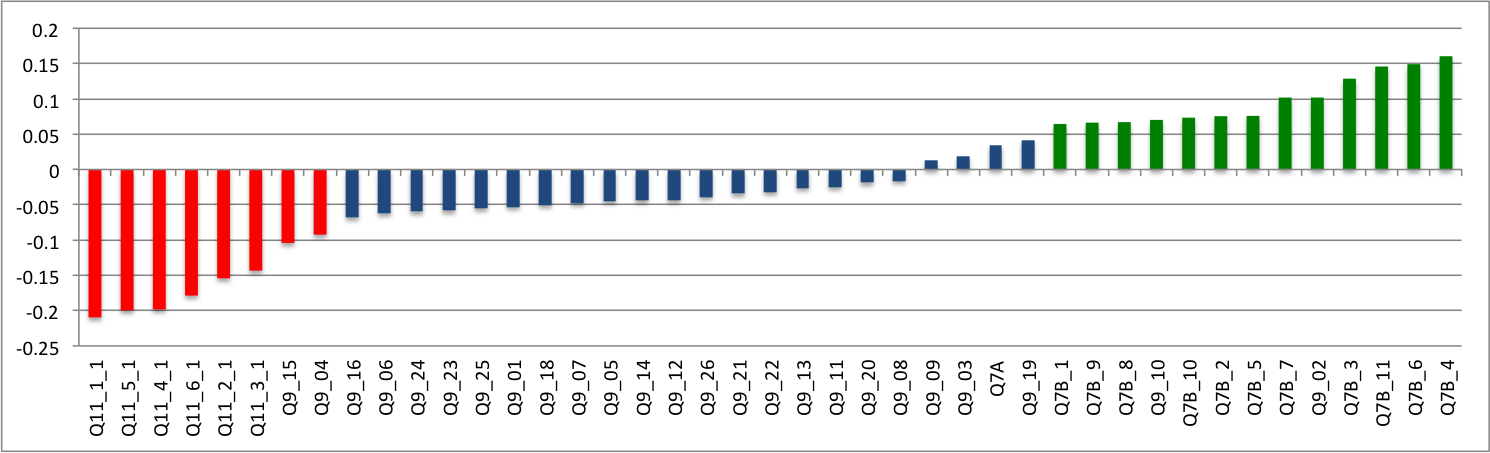
\includegraphics[ width=\textwidth ]{CM1_Cluster6.png}
	\caption{\textbf{CM1 Scores for the 43 questions for Cluster6, based on the
	clustering dataset.} The selected top and bottom questions are shown in red
	and green respectevly.}
	\label{fig:CM1Cluster6}
\end{figure}
\begin{figure}[h]
	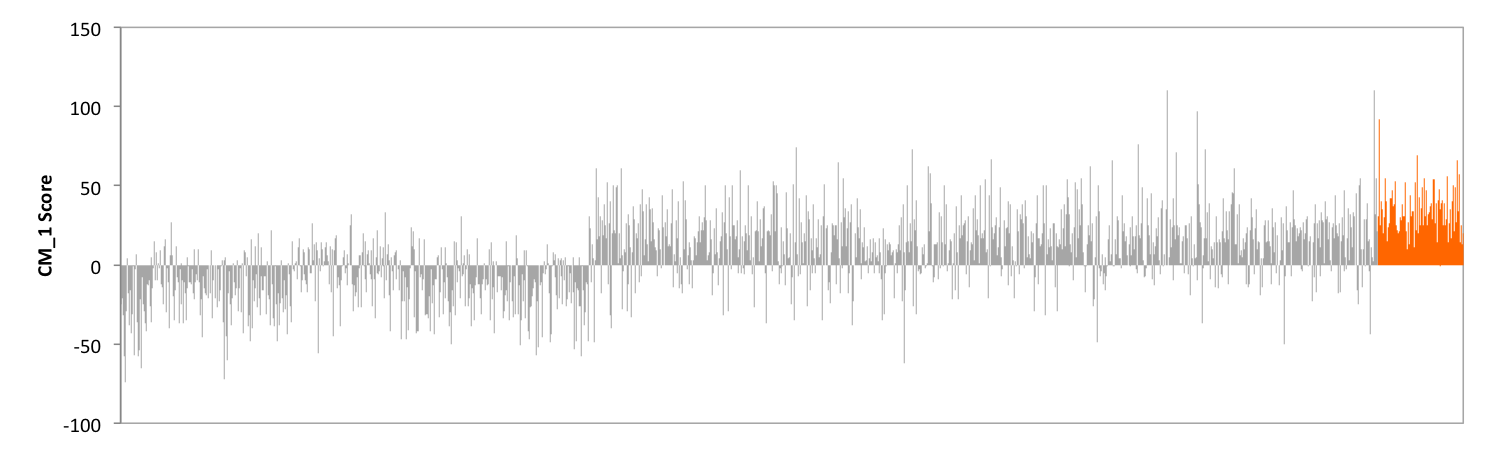
\includegraphics[ width=\textwidth]{Difference_Cluster6.png}
	\caption{\textbf{Difference between the cumulative CM1 scores for Cluster6's 12
	lowest and 13 highest scoring questions} The.}
	\label{fig:DifferencesCluster6}
\end{figure}




\subsubsection{Description of Clusters}


\subsection{Discussion and Conclusion}
%(together)

\bibliography{references}

\end{document}



